\section{Neural Network}

The Convolutional Auto-Encoder was used to de-noise raw data from CLAS12 drift chambers~\cite{Thomadakis:2022zcd}. The input and output for the network are matrices of size 36x112. The training data was extracted from experimental data. The raw hits (converted into a matrix) were used as an input for the neural network and a matrix constructed only from hits that belong to reconstructed tracks an output. In training data set multiple track hits were allowed in the output matrix. The structure of neural network can be seen on Figure~\ref{network:cnn_encoder}.

\begin{figure}[!h]
\begin{center}
 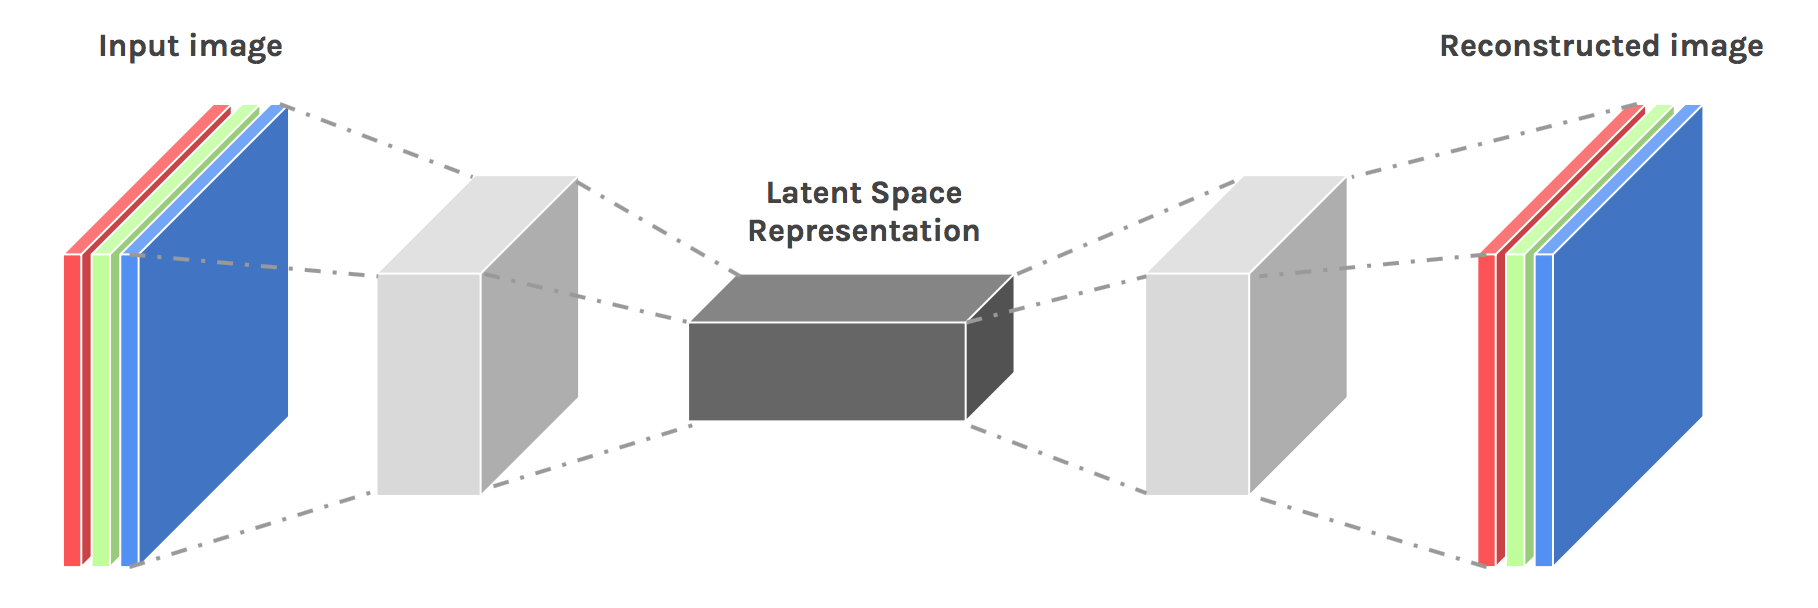
\includegraphics[width=5.1in]{images/convolutional-autoencoder.png}
\caption {De-noising neural network architecture.}
 \label{network:cnn_encoder}
 \end{center}
\end{figure}

The network was validated on experimental data where number of hits along the track trajectory were compared for de-noised data.
Example of comparison can be seen in Figure~\ref{network:cnn_results} where raw data (left column) is shown along with data with hits
belonging to reconstructed track (middle column) and reduced data passing through de-nosing program (right column).

\begin{figure}[!h]
\begin{center}
 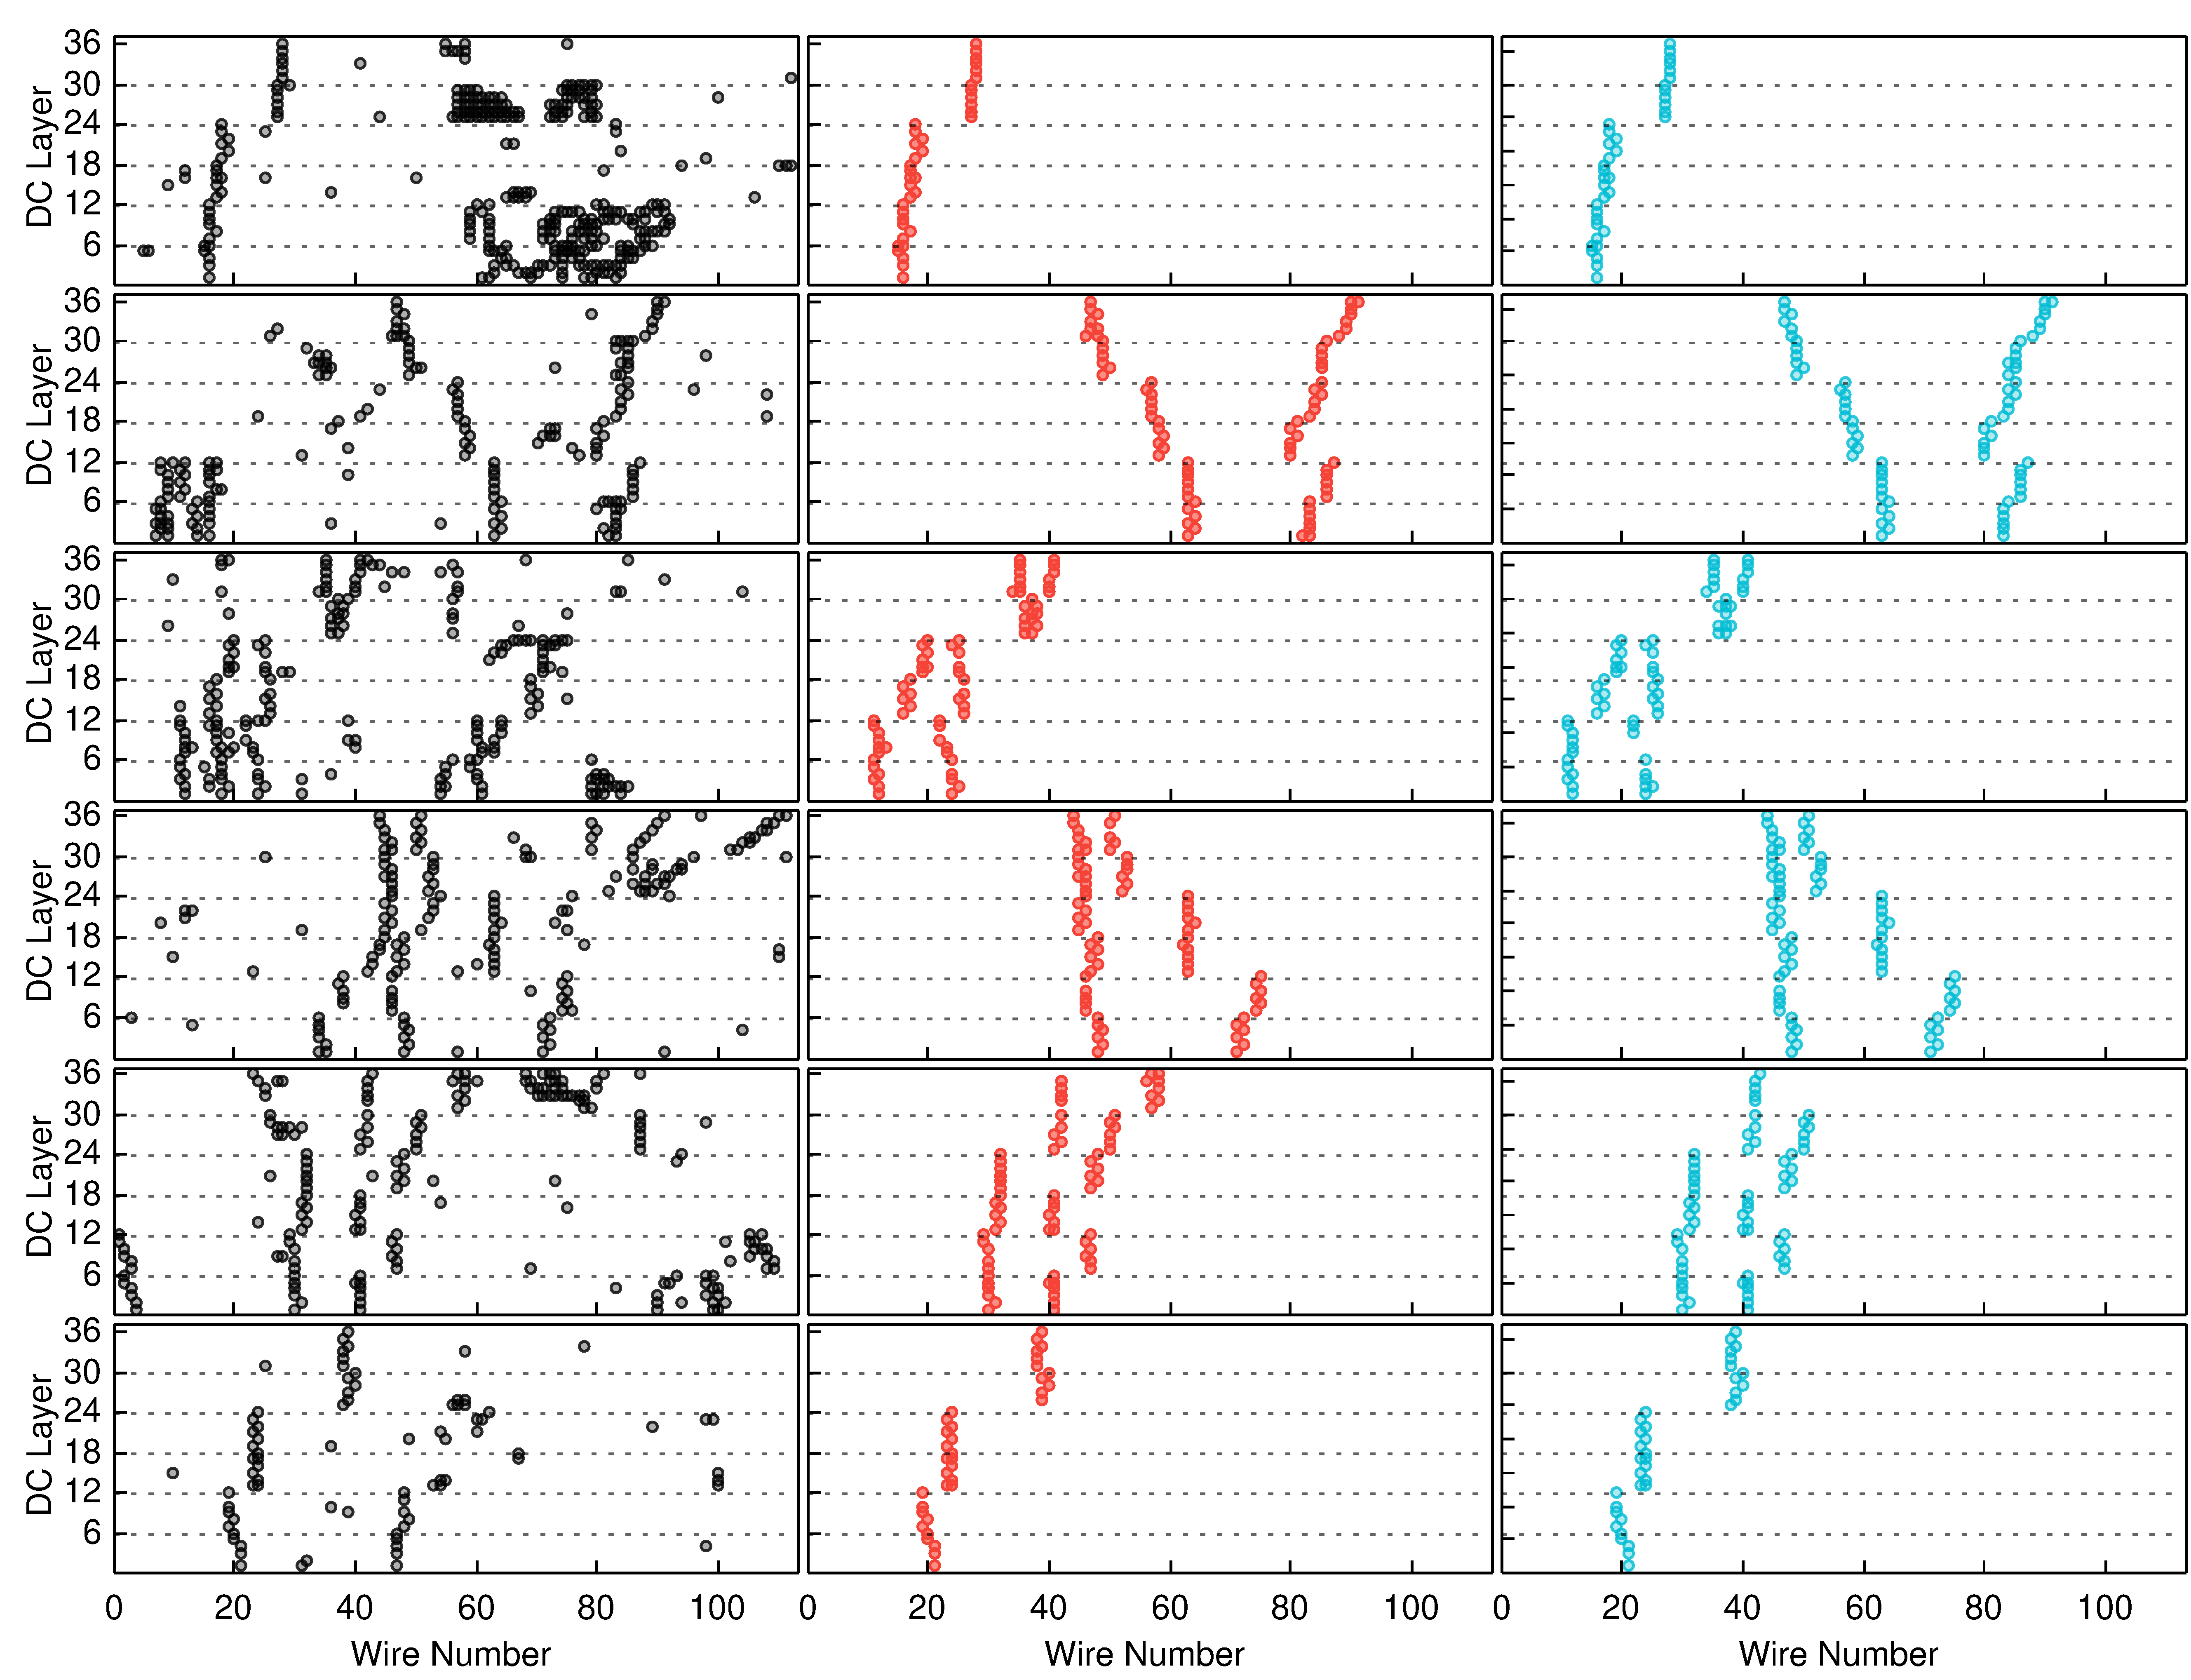
\includegraphics[width=5.8in]{images/cnn_denoise_results.pdf}
\caption {De-noising neural network architecture.}
 \label{network:cnn_results}
 \end{center}
\end{figure}

As can be seen from the figure de-noiser removes all background hits not associated with a track. Systematic studies~\cite{Thomadakis:2022zcd} showed that more than $95\%$ of the track related hits are preserved in the output of de-noiser while background hits are significantly suppressed.

For out implementation we used TensorFlow/Keras~\cite{keras-website} to train and evaluate the network. The resulting network parameters (weights) were saved in HDF5 file. The de-noiser implementation for CLAS12 reconstruction software is done using DeepLearning4J~\cite{dl4j-website} which supports model imports through HDF5 files. The de-noising is not yet implemented as a part of CLAS12 reconstruction workflow, and works as a standalone package to process raw data before analyzing with reconstruction software.
